\providecommand{\placeholderfigure}[3]{%
    \begin{figure}[H]
        \centering
        \fbox{%
            \parbox[c][4.0cm][c]{0.88\textwidth}{%
                \centering
                \textit{#1}%
            }%
        }
        \caption{#2}
        \label{#3}
    \end{figure}
}

\section{HỆ THỐNG CẢM BIẾN VÀ XỬ LÝ DỮ LIỆU}
\label{sec:sensor-data-processing}

Chương này phân tích lớp cảm biến và lớp xử lý dữ liệu của hệ thống robot tự hành TurtleBot4. Khác với Chương 2, nội dung không đi sâu lại vào lý thuyết chung của từng cảm biến mà tập trung vào cách các nguồn dữ liệu được sử dụng trong project: LiDAR cung cấp dữ liệu hình học cho SLAM và costmap; camera RGB-D OAK-D cung cấp ảnh màu, ảnh chiều sâu và thông số nội tại; YOLOv8n xử lý ảnh RGB để phát hiện đối tượng; Object Localization kết hợp bounding box, depth và camera intrinsic để suy ra vị trí 3D; TF/TF2 dùng để đưa dữ liệu về cùng hệ tọa độ phục vụ điều hướng.

\begin{figure}[H]
\centering
\resizebox{\textwidth}{!}{
\begin{tikzpicture}[
  block/.style={draw, rounded corners, fill=cyan!10, align=center, minimum height=1.2cm, text width=3.8cm},
  sensor/.style={draw, circle, fill=orange!10, align=center, minimum size=1.8cm},
  >=Latex
]
\node[sensor] (lidar) at (0, 0) {LiDAR};
\node[sensor] (cam)   at (0, -3.3) {OAK-D};
\node[sensor] (odom)  at (0, -6.6) {Odometry};

\node[block] (slam)  at (4.5, 0) {SLAM / Costmap\\(Dữ liệu hình học)};
\node[block] (yolo)  at (4.5, -2.2) {YOLOv8n\\(Nhận diện)};
\node[block] (depth) at (4.5, -4.4) {Depth Processing\\(Khoảng cách)};

\node[block] (loc)   at (9.5, -3.3) {Object Localization\\(Tọa độ 3D)};

\node[block, fill=green!10] (nav)   at (14.5, -1.6) {Navigation \&\\Mission Manager};

\draw[->, thick] (lidar) -- node[above, font=\footnotesize] {/scan} (slam);
\draw[->, thick] (cam.east) -- +(0.5,0) |- node[pos=0.75, above, font=\footnotesize] {RGB} (yolo.west);
\draw[->, thick] (cam.east) -- +(0.5,0) |- node[pos=0.75, below, font=\footnotesize] {Depth} (depth.west);

\draw[->, thick] (yolo.east) -| (loc.north);
\draw[->, thick] (depth.east) -| (loc.south);

\draw[->, thick] (slam.east) -| (nav.north);
\draw[->, thick] (loc.east) -| ([xshift=-0.5cm]nav.south);

\draw[->, thick] (odom.east) -| node[near start, below, font=\footnotesize] {/odom} ([xshift=0.5cm]nav.south);
\end{tikzpicture}
}
\caption{Sơ đồ tổng quan pipeline cảm biến và xử lý dữ liệu trong TurtleBot4}
\label{fig:sensor-processing-pipeline}
\end{figure}

\subsection{Vai trò của cảm biến trong đề tài}
\label{subsec:sensor-role}

Trong hệ robot tự hành, cảm biến là nguồn thông tin đầu vào quyết định robot biết gì về môi trường và trạng thái của chính nó. Nếu thiếu cảm biến, robot chỉ có thể chạy theo lệnh cố định mà không biết vật cản, vị trí bản thân hay vị trí mục tiêu. Trong project TurtleBot4, cảm biến được dùng cho ba nhóm nhiệm vụ chính: nhận biết không gian xung quanh, nhận diện mục tiêu và hỗ trợ điều hướng.

\begin{table}[H]
    \centering
    \caption{Các nhóm dữ liệu cảm biến sử dụng trong project}
    \label{tab:sensor-data-groups}
    \renewcommand{\arraystretch}{1.25}
    \small
    \begin{tabularx}{\textwidth}{|>{\raggedright\arraybackslash}p{0.23\textwidth}|>{\raggedright\arraybackslash}p{0.25\textwidth}|>{\raggedright\arraybackslash}X|}
        \hline
        \textbf{Nhóm dữ liệu} & \textbf{Nguồn dữ liệu} & \textbf{Mục đích sử dụng trong project} \\
        \hline
        Dữ liệu hình học & LiDAR \texttt{/scan} & Xây dựng bản đồ, tránh vật cản và tạo costmap cho Nav2. \\
        \hline
        Dữ liệu chuyển động & Odometry \texttt{/odom} & Ước lượng chuyển động tương đối của robot theo thời gian. \\
        \hline
        Dữ liệu thị giác & Ảnh RGB từ OAK-D & Đưa vào YOLOv8n để phát hiện người hoặc đối tượng mục tiêu. \\
        \hline
        Dữ liệu chiều sâu & Depth image từ OAK-D & Tính khoảng cách từ camera đến vùng chứa mục tiêu. \\
        \hline
        Dữ liệu hình học hệ tọa độ & TF/TF2 & Chuyển đổi pose giữa \texttt{camera}, \texttt{base\_link}, \texttt{odom} và \texttt{map}. \\
        \hline
    \end{tabularx}
\end{table}

Luồng xử lý cảm biến trong chương này có thể hiểu theo chuỗi: đo dữ liệu thô, kiểm tra dữ liệu, chuyển đổi dữ liệu sang dạng ROS2 topic, xử lý thành thông tin có ý nghĩa, rồi đưa thông tin này cho các module điều hướng và điều phối nhiệm vụ.

\begin{figure}[H]
\centering
\begin{tikzpicture}[
  node distance=2.5cm,
  block/.style={draw, rectangle, fill=blue!5, align=center, minimum height=1.2cm, minimum width=2.5cm, thick},
  >=Latex
]
\node[block, fill=orange!10] (sensor) {Cảm biến\\(Sense)};
\node[block, right=of sensor] (process) {Xử lý / Lập kế hoạch\\(Think)};
\node[block, below=of process] (control) {Điều khiển\\(Act)};
\node[block, left=of control] (env) {Môi trường\\(Environment)};

\draw[->, thick] (env) -- node[left, font=\footnotesize] {Tín hiệu vật lý} (sensor);
\draw[->, thick] (sensor) -- node[above, font=\footnotesize] {Dữ liệu thô} (process);
\draw[->, thick] (process) -- node[right, font=\footnotesize] {Lệnh vận tốc} (control);
\draw[->, thick] (control) -- node[below, font=\footnotesize] {Hành động} (env);
\end{tikzpicture}
\caption{Vị trí của lớp cảm biến trong vòng kín cảm biến -- xử lý -- điều khiển -- chấp hành}
\label{fig:sensor-layer-feedback-loop}
\end{figure}

\subsection{LiDAR và dữ liệu /scan}
\label{subsec:lidar-scan}

\subsubsection{Chức năng của LiDAR trong hệ thống}
\label{subsubsec:lidar-function}

LiDAR là cảm biến chính phục vụ nhận biết hình học xung quanh robot. Trong project, dữ liệu LiDAR được publish dưới dạng topic \texttt{/scan}. Topic này được SLAM Toolbox dùng để xây dựng bản đồ và được Nav2 dùng để cập nhật costmap, từ đó giúp robot tránh vật cản trong quá trình di chuyển.

\begin{table}[H]
    \centering
    \caption{Vai trò của LiDAR trong hệ thống}
    \label{tab:lidar-role}
    \renewcommand{\arraystretch}{1.25}
    \small
    \begin{tabularx}{\textwidth}{|>{\raggedright\arraybackslash}p{0.25\textwidth}|>{\raggedright\arraybackslash}X|}
        \hline
        \textbf{Mục} & \textbf{Nội dung} \\
        \hline
        Input của LiDAR & Môi trường xung quanh robot, gồm tường, kệ hàng, vật cản và bề mặt phản xạ laser. \\
        \hline
        Output của LiDAR & Bản tin \texttt{LaserScan} trên topic \texttt{/scan}. \\
        \hline
        Dạng dữ liệu & Mảng khoảng cách theo từng góc quét trong mặt phẳng ngang. \\
        \hline
        Module sử dụng & SLAM Toolbox, Nav2 costmap, RViz để hiển thị \texttt{LaserScan}. \\
        \hline
        Vai trò trong project & Tạo thông tin khoảng cách giúp robot lập bản đồ, định vị và tránh vật cản. \\
        \hline
    \end{tabularx}
\end{table}

\subsubsection{Cách hoạt động và cách tính dữ liệu LiDAR}
\label{subsubsec:lidar-calculation}

Một phép đo LiDAR có thể được mô tả bằng cặp giá trị gồm góc quét và khoảng cách. Với mỗi hướng quét, cảm biến phát tia laser ra môi trường, nhận tín hiệu phản xạ quay lại, sau đó tính khoảng cách đến vật cản. Nếu dùng nguyên lý thời gian bay, khoảng cách có thể được tính theo công thức:

\begin{equation}
    d = \frac{c\,\Delta t}{2}
    \label{eq:lidar-time-of-flight}
\end{equation}

Trong đó, $d$ là khoảng cách từ cảm biến đến vật cản, $c$ là tốc độ lan truyền của ánh sáng, $\Delta t$ là thời gian từ lúc phát tia đến lúc nhận tín hiệu phản xạ. Hệ số $2$ xuất hiện vì tia laser đi từ cảm biến đến vật cản rồi phản xạ quay lại cảm biến, tức là quãng đường đo được gấp đôi khoảng cách thực.

Trong bản tin \texttt{LaserScan}, mỗi phần tử khoảng cách tương ứng với một góc quét. Nếu gọi $\theta_i$ là góc của tia quét thứ $i$, khoảng cách đo được là $r_i$, tọa độ điểm vật cản trong hệ tọa độ LiDAR có thể biểu diễn là:

\begin{equation}
    x_i = r_i\cos(\theta_i), \qquad
    y_i = r_i\sin(\theta_i)
    \label{eq:lidar-polar-to-cartesian}
\end{equation}

Công thức trên biến dữ liệu cực của LiDAR thành điểm trong mặt phẳng hai chiều. Các điểm này được dùng để tạo hình dạng tường, vật cản và vùng trống trong bản đồ occupancy grid. Trong cấu hình của đề tài, các tham số quan trọng gồm \texttt{resolution = 0.05 m}, \texttt{min\_laser\_range = 0.2 m} và \texttt{max\_laser\_range = 12.0 m}. Các giá trị nằm ngoài dải đo hợp lệ sẽ bị loại bỏ hoặc không được dùng trong SLAM và costmap.

\begin{figure}[H]
    \centering
    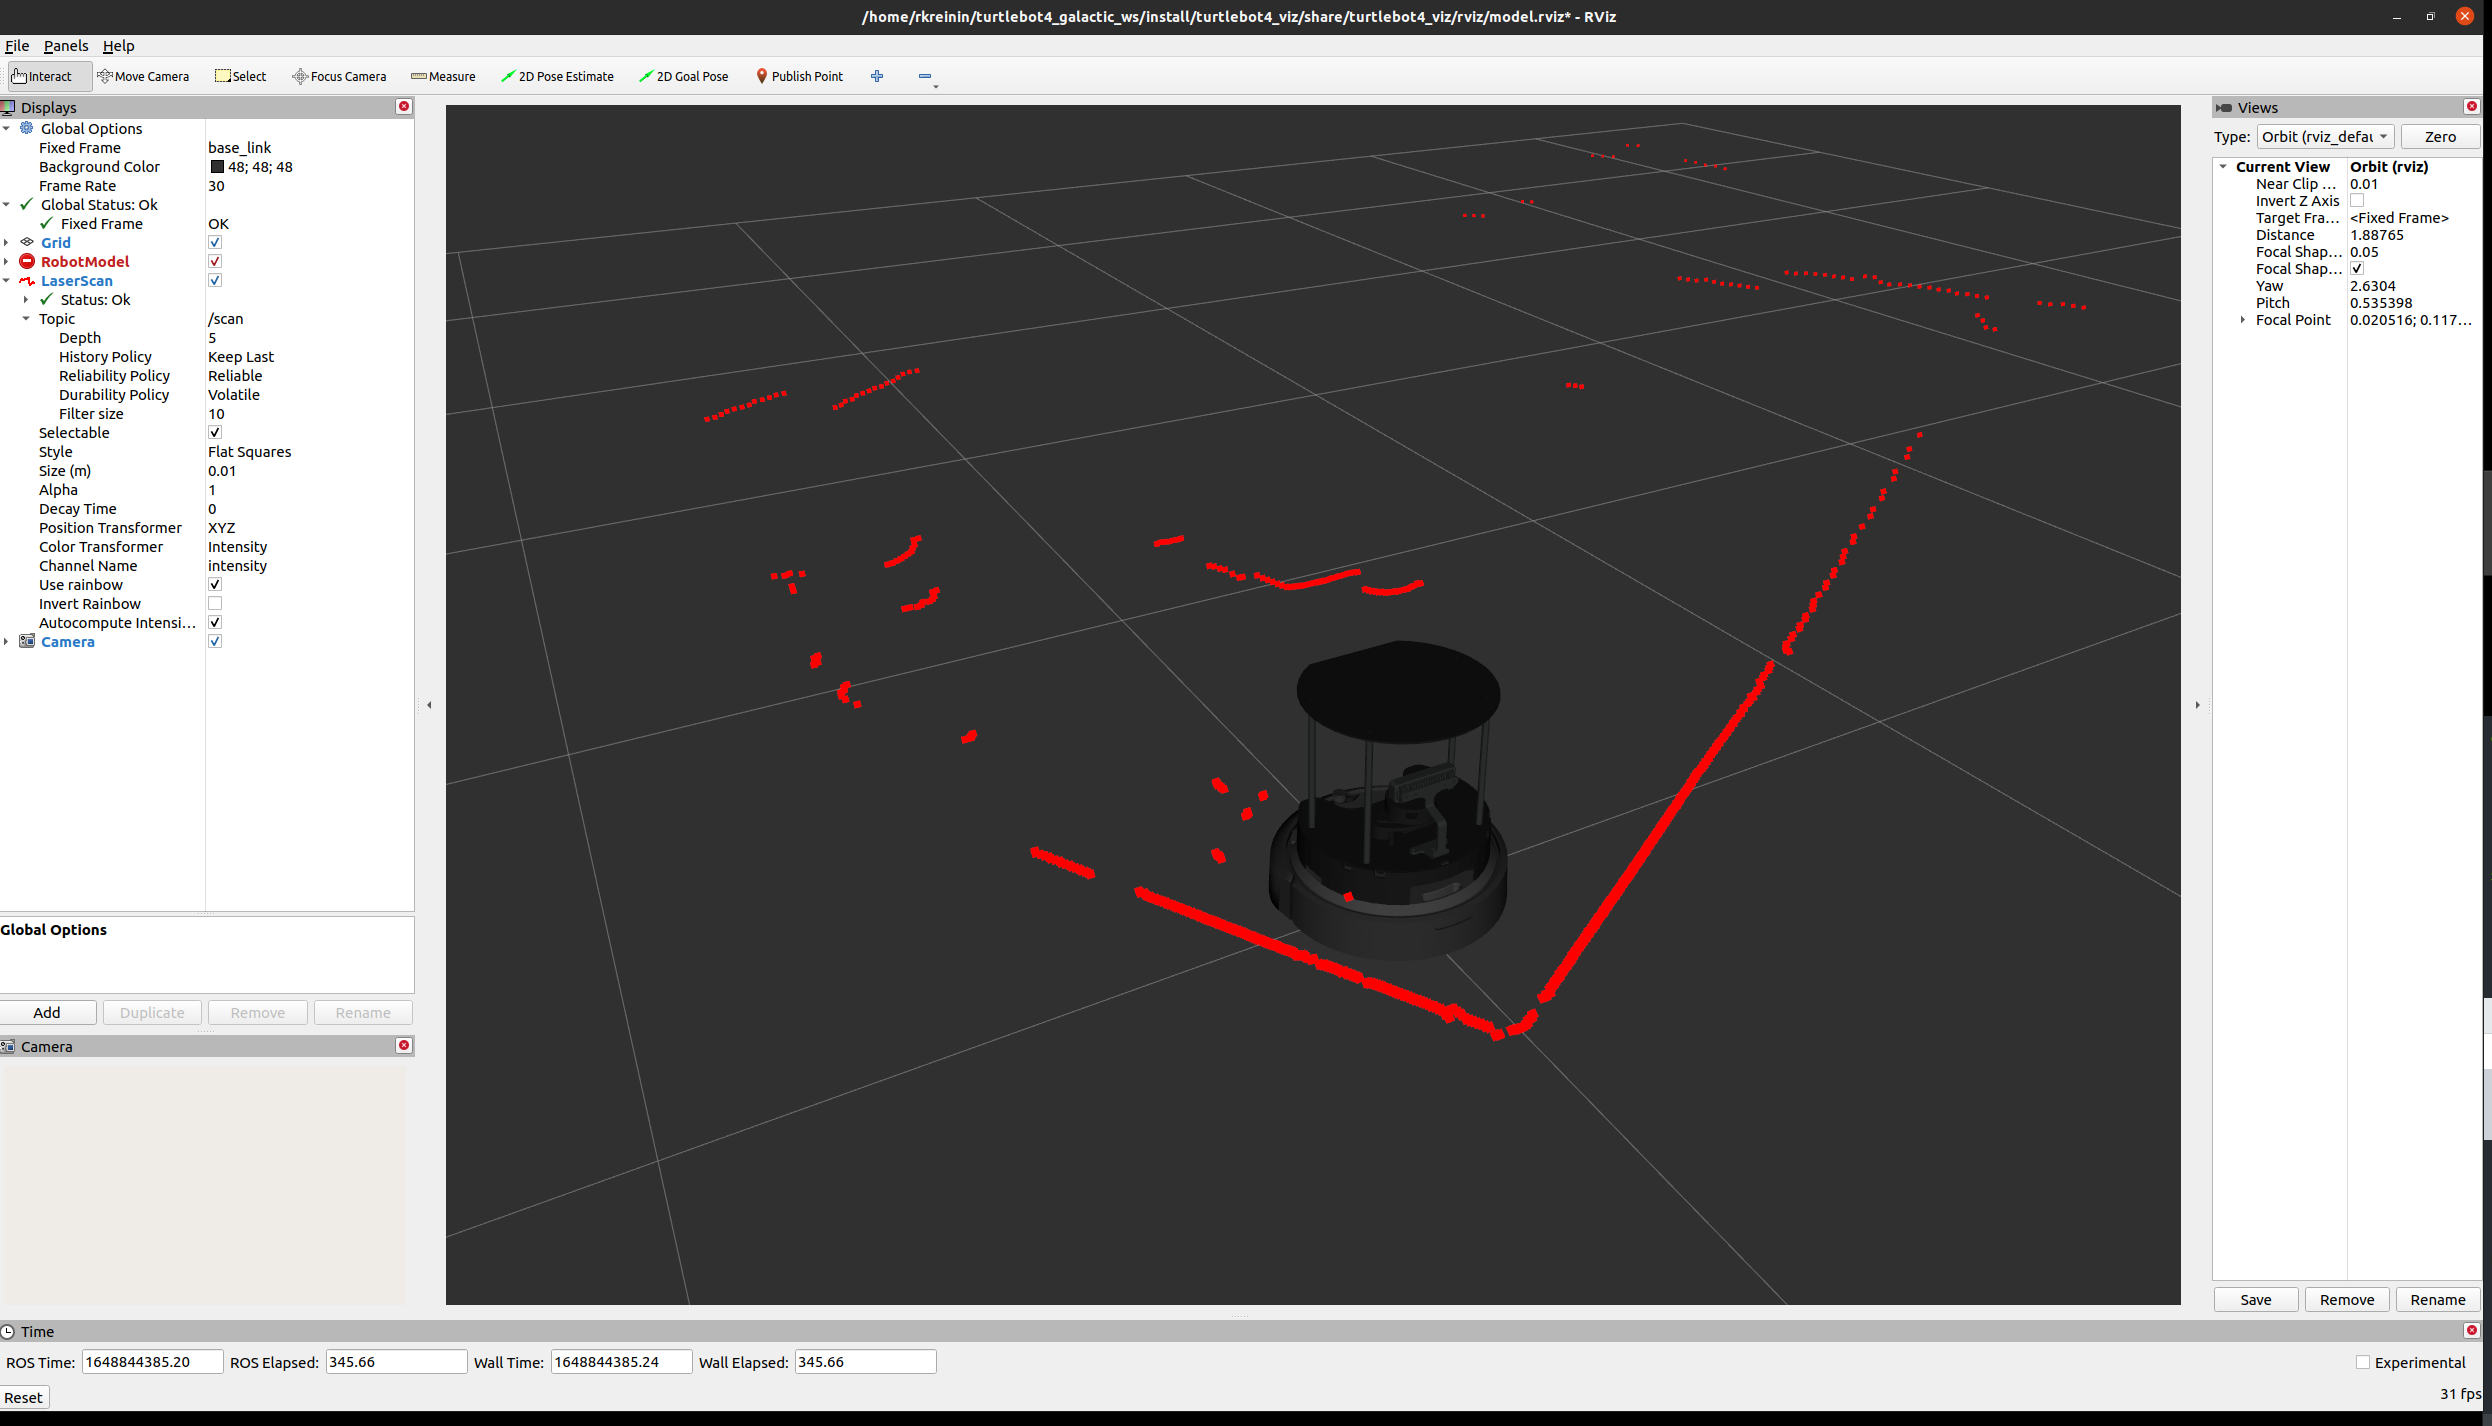
\includegraphics[width=0.7\textwidth]{images/chapter4/laserscan.png}
    \caption{Minh họa LiDAR 2D quét môi trường và tạo tập điểm khoảng cách}
    \label{fig:lidar-2d-scan}
\end{figure}

\subsubsection{Kiểm tra và lỗi thường gặp của dữ liệu /scan}
\label{subsubsec:lidar-troubleshooting}

Trong mô phỏng, dữ liệu \texttt{/scan} có thể bất thường nếu frame LiDAR đặt sai, mô hình collision che tia laser, hoặc topic chưa được bridge đúng giữa Gazebo/Ignition và ROS2. Khi \texttt{/scan} có giá trị gần như cố định hoặc không thay đổi theo môi trường, robot có thể xây dựng bản đồ sai, costmap sai và điều hướng không ổn định.

\begin{table}[H]
    \centering
    \caption{Một số lỗi thường gặp của dữ liệu \texttt{/scan}}
    \label{tab:scan-errors}
    \renewcommand{\arraystretch}{1.25}
    \small
    \begin{tabularx}{\textwidth}{|>{\raggedright\arraybackslash}p{0.22\textwidth}|>{\raggedright\arraybackslash}p{0.34\textwidth}|>{\raggedright\arraybackslash}X|}
        \hline
        \textbf{Hiện tượng} & \textbf{Nguyên nhân có thể} & \textbf{Cách kiểm tra} \\
        \hline
        Không có dữ liệu \texttt{/scan} & LiDAR chưa spawn, bridge chưa hoạt động hoặc sai namespace. & Chạy \texttt{ros2 topic echo /scan --once} và kiểm tra danh sách topic. \\
        \hline
        Khoảng cách gần như cố định & LiDAR bị che bởi mô hình robot hoặc collision không đúng. & Quan sát \texttt{LaserScan} trong RViz và kiểm tra frame \texttt{rplidar\_link}. \\
        \hline
        Scan lệch hướng & Sai quan hệ TF giữa \texttt{rplidar\_link} và \texttt{base\_link}. & Hiển thị TF trong RViz và kiểm tra trục tọa độ. \\
        \hline
        SLAM tạo bản đồ méo & Odometry, scan hoặc TF không đồng bộ. & Kiểm tra \texttt{/odom}, \texttt{/scan}, \texttt{/clock} và transform \texttt{map -> odom -> base\_link}. \\
        \hline
    \end{tabularx}
\end{table}

\subsection{Camera RGB-D OAK-D}
\label{subsec:rgbd-camera}

\subsubsection{Chức năng của camera RGB-D trong project}
\label{subsubsec:rgbd-function}

Camera RGB-D OAK-D cung cấp hai loại thông tin bổ sung cho nhau. Ảnh RGB chứa thông tin màu sắc và hình dạng, phù hợp cho nhận diện đối tượng bằng YOLOv8n. Ảnh depth chứa khoảng cách của từng điểm ảnh đến camera, giúp hệ thống xác định mục tiêu ở gần hay xa. Ngoài ra, bản tin \texttt{camera\_info} cung cấp các tham số nội tại của camera để chuyển đổi từ điểm ảnh 2D sang tọa độ 3D.

\begin{table}[H]
    \centering
    \caption{Các topic liên quan đến camera RGB-D và định vị mục tiêu}
    \label{tab:rgbd-topics}
    \renewcommand{\arraystretch}{1.25}
    \small
    \begin{tabularx}{\textwidth}{|>{\raggedright\arraybackslash}p{0.38\textwidth}|>{\raggedright\arraybackslash}p{0.22\textwidth}|>{\raggedright\arraybackslash}X|}
        \hline
        \textbf{Topic} & \textbf{Loại dữ liệu} & \textbf{Ý nghĩa trong project} \\
        \hline
        \texttt{/oakd/rgb/preview/}\newline\texttt{image\_raw} & Ảnh RGB & Đầu vào cho node YOLOv8n để phát hiện đối tượng. \\
        \hline
        \texttt{/oakd/rgb/preview/}\newline\texttt{depth} & Ảnh chiều sâu & Cung cấp khoảng cách $Z$ tại vùng chứa mục tiêu. \\
        \hline
        \texttt{/oakd/rgb/preview/}\newline\texttt{camera\_info} & Thông số nội tại camera & Cung cấp $f_x$, $f_y$, $c_x$, $c_y$ để tính tọa độ 3D. \\
        \hline
        \texttt{/vision/}\newline\texttt{detected\_objects} & \texttt{Detection-}\newline\texttt{2DArray} & Output của YOLOv8n, gồm bounding box, class id và confidence. \\
        \hline
        \texttt{/target\_object\_pose\_map} & \texttt{PoseStamped} & Output của bước định vị, biểu diễn pose mục tiêu để Mission Manager sử dụng. \\
        \hline
        \texttt{/target\_object\_marker} & \texttt{Marker} & Dùng để hiển thị vị trí mục tiêu trong RViz. \\
        \hline
    \end{tabularx}
\end{table}

\subsubsection{Thành phần dữ liệu của camera RGB-D}
\label{subsubsec:rgbd-components}

\begin{table}[H]
    \centering
    \caption{Thành phần dữ liệu của camera RGB-D}
    \label{tab:rgbd-components}
    \renewcommand{\arraystretch}{1.25}
    \small
    \begin{tabularx}{\textwidth}{|>{\raggedright\arraybackslash}p{0.28\textwidth}|>{\raggedright\arraybackslash}X|}
        \hline
        \textbf{Thành phần} & \textbf{Chức năng} \\
        \hline
        Camera RGB & Thu ảnh màu của môi trường, giúp nhận diện người hoặc đối tượng bằng mô hình học sâu. \\
        \hline
        Cảm biến depth hoặc mô phỏng depth & Tạo ảnh chiều sâu, trong đó mỗi pixel biểu diễn khoảng cách từ camera đến bề mặt quan sát được. \\
        \hline
        \texttt{CameraInfo} & Lưu thông số nội tại như $f_x$, $f_y$, $c_x$, $c_y$ và kích thước ảnh. \\
        \hline
        Node xử lý ảnh & Nhận ảnh, chuyển đổi định dạng và đưa vào mô hình nhận diện. \\
        \hline
        Giao tiếp ROS2 & Publish/subscribe dữ liệu camera qua các topic ROS2 để các node khác sử dụng. \\
        \hline
    \end{tabularx}
\end{table}

\subsubsection{Cách tính tọa độ 3D từ ảnh RGB-D}
\label{subsubsec:rgbd-3d-calculation}

Sau khi YOLOv8n phát hiện đối tượng, hệ thống lấy tâm bounding box trên ảnh RGB. Giả sử tâm bounding box là điểm ảnh có tọa độ $(u, v)$. Từ ảnh depth, lấy giá trị độ sâu tại vùng lân cận điểm này. Để giảm nhiễu, hệ thống không nên lấy một pixel duy nhất mà nên lấy trung vị của một vùng nhỏ xung quanh tâm bbox. Gọi giá trị depth hợp lệ là $Z$.

Theo mô hình camera lỗ kim, điểm ảnh 2D có thể được chuyển sang tọa độ 3D trong hệ camera bằng các công thức:

\begin{align}
    X_c &= \frac{(u-c_x)Z}{f_x}, \label{eq:rgbd-xc}\\
    Y_c &= \frac{(v-c_y)Z}{f_y}, \label{eq:rgbd-yc}\\
    Z_c &= Z. \label{eq:rgbd-zc}
\end{align}

Trong đó, $u$, $v$ là tọa độ pixel của tâm bbox; $Z$ là độ sâu tại vùng tâm bbox; $f_x$ và $f_y$ là tiêu cự theo đơn vị pixel; $c_x$ và $c_y$ là tọa độ tâm ảnh. Nếu $u=c_x$ và $v=c_y$, mục tiêu nằm gần trục quang học của camera. Nếu $u$ lệch khỏi $c_x$, mục tiêu lệch ngang trong ảnh; nếu $v$ lệch khỏi $c_y$, mục tiêu lệch theo phương dọc ảnh.

Do quy ước trục của camera khác quy ước trục của robot trong ROS, tọa độ trong hệ camera cần được ánh xạ sang quy ước ROS như sau:

\begin{equation}
    x_{\mathrm{ros}} = Z_c, \qquad
    y_{\mathrm{ros}} = -X_c, \qquad
    z_{\mathrm{ros}} = -Y_c
    \label{eq:camera-to-ros-axis}
\end{equation}

Cách ánh xạ này giúp hướng phía trước camera tương ứng với trục $x$ của robot trong ROS. Kết quả cuối cùng là một pose mục tiêu tương đối so với camera hoặc so với frame đã được biến đổi bằng TF.

\begin{figure}[H]
\centering
\begin{tikzpicture}[
  >=Latex,
  font=\small
]
% Camera center
\filldraw[black] (0,0) circle (2pt) node[anchor=north] {Tâm quang học $O$};

% Image plane
\draw[thick, fill=blue!5, opacity=0.8] (2,-1.5) -- (2,1.5) -- (3,2) -- (3,-1) -- cycle;
\node at (2.5, 1.8) {Mặt phẳng ảnh};

% Principal point
\filldraw[red] (2.5, 0.25) circle (1.5pt) node[anchor=north] {$(c_x, c_y)$};

% Pixel point
\filldraw[blue] (2.2, 1.0) circle (1.5pt) node[anchor=south] {$(u, v)$};

% 3D point
\filldraw[green!50!black] (6.6, 3.0) circle (2pt) node[anchor=south] {Mục tiêu $(X_c, Y_c, Z_c)$};

% Optical axis
\draw[dashed, thick] (0,0) -- (8,0) node[anchor=west] {$Z_c$};

% Rays
\draw[thick] (0,0) -- (6.6, 3.0);

% Labels
\draw[<->] (0,-0.5) -- (2.5,-0.5) node[midway, below] {Tiêu cự $f$};
\draw[<->] (2.5, 0.25) -- (2.2, 1.0) node[midway, left] {$\Delta p$};
\end{tikzpicture}
\caption{Mô hình camera pinhole và cách chuyển điểm ảnh RGB-D sang tọa độ 3D}
\label{fig:rgbd-pinhole-model}
\end{figure}

\subsection{Nhận diện đối tượng bằng YOLOv8n}
\label{subsec:yolov8n-detection}

\subsubsection{Vai trò của YOLOv8n}
\label{subsubsec:yolov8n-role}

YOLOv8n là module nhận diện đối tượng trong project. Node \texttt{tb4\_vision\_oak} nhận ảnh RGB từ camera OAK-D, chạy mô hình YOLOv8n, sau đó xuất ra danh sách đối tượng phát hiện được. Kết quả này không trực tiếp điều khiển robot mà được chuyển cho Object Localization để kết hợp với depth.

\begin{table}[H]
    \centering
    \caption{Input, output và vai trò của YOLOv8n}
    \label{tab:yolov8n-role}
    \renewcommand{\arraystretch}{1.25}
    \small
    \begin{tabularx}{\textwidth}{|>{\raggedright\arraybackslash}p{0.24\textwidth}|>{\raggedright\arraybackslash}X|}
        \hline
        \textbf{Mục} & \textbf{Nội dung} \\
        \hline
        Input & Ảnh RGB từ \texttt{/oakd/rgb/preview/image\_raw}. \\
        \hline
        Xử lý & Chạy inference bằng mô hình YOLOv8n, lọc detection theo confidence. \\
        \hline
        Output & \texttt{Detection2DArray} trên \texttt{/vision/detected\_objects}. \\
        \hline
        Thông tin trong output & Tâm bbox, kích thước bbox, class id, confidence. \\
        \hline
        Ứng dụng trong project & Phát hiện mục tiêu, ưu tiên class \texttt{person} nếu xuất hiện. \\
        \hline
    \end{tabularx}
\end{table}

\subsubsection{Dữ liệu detection và tiêu chí chọn mục tiêu}
\label{subsubsec:detection-selection}

Mỗi detection có thể được biểu diễn bởi một bounding box và thông tin phân loại. Gọi bounding box có tâm là $(u, v)$, chiều rộng $w$ và chiều cao $h$. Vùng bbox được mô tả bởi:

\begin{equation}
    B = \left(u,\, v,\, w,\, h,\, \texttt{class\_id},\, \mathrm{conf}\right)
    \label{eq:bbox-format}
\end{equation}

Trong đó, \texttt{class\_id} cho biết lớp đối tượng, còn $\mathrm{conf}$ là độ tin cậy của dự đoán. Nếu có nhiều detection, hệ thống có thể áp dụng quy tắc chọn mục tiêu như sau: ưu tiên đối tượng thuộc lớp \texttt{person}; nếu không có \texttt{person}, chọn detection có confidence cao nhất; nếu confidence thấp hơn ngưỡng, không tạo mục tiêu.

\begin{equation}
    B_{\mathrm{target}}
    =
    \underset{i}{\arg\max}\; \mathrm{conf}_i,
    \qquad \mathrm{conf}_i \geq \tau
    \label{eq:target-bbox-selection}
\end{equation}

Trong công thức trên, $\tau$ là ngưỡng confidence. Trong project, ngưỡng mặc định là $0.5$. Việc dùng ngưỡng giúp loại bỏ các phát hiện không chắc chắn, tránh việc Mission Manager phản ứng sai với nhiễu hoặc vật thể không mong muốn.

\begin{figure}[H]
    \centering
    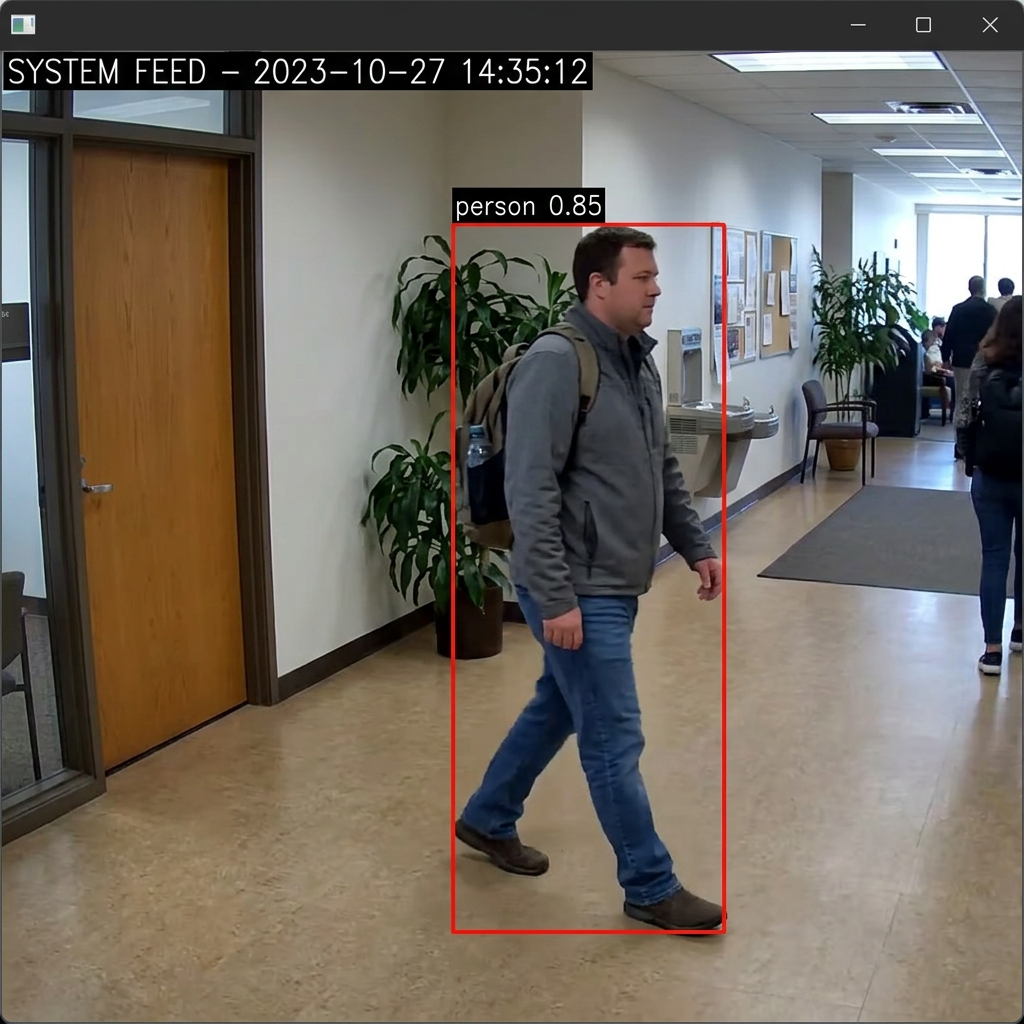
\includegraphics[width=0.6\textwidth]{images/chapter4/yolo_detection.png}
    \caption{Minh họa YOLOv8n phát hiện bounding box trên ảnh RGB}
    \label{fig:yolov8n-bbox}
\end{figure}

\subsection{Định vị mục tiêu từ RGB-D}
\label{subsec:rgbd-object-localization}

\subsubsection{Quy trình định vị}
\label{subsubsec:localization-process}

Định vị mục tiêu là bước biến thông tin nhận diện 2D thành vị trí 3D có thể dùng cho điều hướng. Nếu chỉ có YOLOv8n, robot chỉ biết mục tiêu nằm ở đâu trong ảnh. Nếu chỉ có depth, robot không biết vùng nào là mục tiêu. Vì vậy, cần kết hợp bbox từ YOLOv8n với ảnh depth và thông số camera.

\begin{table}[H]
    \centering
    \caption{Quy trình định vị mục tiêu từ dữ liệu RGB-D}
    \label{tab:rgbd-localization-process}
    \renewcommand{\arraystretch}{1.25}
    \small
    \begin{tabularx}{\textwidth}{|>{\centering\arraybackslash}p{0.08\textwidth}|>{\raggedright\arraybackslash}p{0.28\textwidth}|>{\raggedright\arraybackslash}X|}
        \hline
        \textbf{Bước} & \textbf{Dữ liệu sử dụng} & \textbf{Kết quả} \\
        \hline
        1 & \texttt{Detection2DArray} & Chọn bbox mục tiêu. \\
        \hline
        2 & Ảnh depth & Lấy độ sâu $Z$ tại vùng tâm bbox. \\
        \hline
        3 & \texttt{CameraInfo} & Lấy $f_x$, $f_y$, $c_x$, $c_y$. \\
        \hline
        4 & Công thức pinhole & Tính tọa độ 3D trong hệ camera. \\
        \hline
        5 & TF/TF2 & Chuyển pose sang frame phù hợp như \texttt{map} hoặc \texttt{base\_link}. \\
        \hline
        6 & ROS2 topic & Publish \texttt{/target\_object\_pose\_map} và \texttt{/target\_object\_marker}. \\
        \hline
    \end{tabularx}
\end{table}

\subsubsection{Lọc depth tại vùng bbox}
\label{subsubsec:depth-filtering}

Ảnh depth thường có nhiễu, điểm mất dữ liệu hoặc giá trị không hợp lệ tại biên vật thể. Vì vậy, thay vì lấy đúng một pixel tại tâm bbox, node định vị nên lấy một cửa sổ nhỏ quanh tâm bbox và tính trung vị. Gọi tập giá trị depth hợp lệ trong cửa sổ là $\mathcal{S}$. Giá trị depth dùng để định vị được tính là:

\begin{equation}
    Z = \operatorname{median}\left(\mathcal{S}\right)
    \label{eq:median-depth}
\end{equation}

Cách dùng trung vị giúp giảm ảnh hưởng của các điểm bất thường. Ví dụ, nếu trong cửa sổ có một vài pixel lỗi bằng $0$ hoặc quá lớn, giá trị trung vị vẫn thường ổn định hơn giá trị trung bình hoặc một pixel đơn lẻ.

\begin{table}[H]
    \centering
    \caption{Cách xử lý một số trường hợp depth bất thường}
    \label{tab:depth-filtering-cases}
    \renewcommand{\arraystretch}{1.25}
    \small
    \begin{tabularx}{\textwidth}{|>{\raggedright\arraybackslash}p{0.28\textwidth}|>{\raggedright\arraybackslash}X|}
        \hline
        \textbf{Loại giá trị depth} & \textbf{Cách xử lý đề xuất} \\
        \hline
        $Z=0$ hoặc không hợp lệ & Bỏ qua detection, không publish pose mục tiêu. \\
        \hline
        $Z$ quá nhỏ & Có thể là vật thể quá gần hoặc lỗi đo; cần kiểm tra ngưỡng an toàn. \\
        \hline
        $Z$ quá lớn & Có thể nằm ngoài tầm quan sát hữu ích; không nên dùng để tiếp cận. \\
        \hline
        $Z$ ổn định trong nhiều frame & Có thể dùng để tạo pose mục tiêu tin cậy hơn. \\
        \hline
    \end{tabularx}
\end{table}

\begin{figure}[H]
\centering
\begin{tikzpicture}[>=Latex]
% Bounding box
\draw[thick, blue] (0,0) rectangle (4,6);
\node[blue] at (2, 6.3) {Bounding Box};

% Center point
\filldraw[red] (2,3) circle (2pt) node[anchor=south west] {Tâm $(u, v)$};

% Depth window
\draw[thick, red, dashed] (1.5, 2.5) rectangle (2.5, 3.5);

% Magnified window
\draw[thick, red] (6, 1.5) rectangle (9, 4.5);
\draw[dashed, gray] (2.5, 3.5) -- (6, 4.5);
\draw[dashed, gray] (2.5, 2.5) -- (6, 1.5);

% Pixels in magnified window
\draw[step=1cm, gray, very thin] (6,1.5) grid (9,4.5);
\node at (6.5, 4.0) {1.5}; \node at (7.5, 4.0) {1.6}; \node at (8.5, 4.0) {1.5};
\node at (6.5, 3.0) {1.5}; \node at (7.5, 3.0) {0.0}; \node at (8.5, 3.0) {1.6};
\node at (6.5, 2.0) {1.4}; \node at (7.5, 2.0) {1.5}; \node at (8.5, 2.0) {5.0};

\node[align=center] at (7.5, 0.5) {$\mathcal{S} = \{0.0, 1.4, 1.5, 1.5, 1.5, 1.5, 1.6, 1.6, 5.0\}$\\[0.2cm] $\operatorname{median}(\mathcal{S}) = 1.5\,$m};
\end{tikzpicture}
\caption{Minh họa lấy depth trung vị trong cửa sổ quanh tâm bounding box}
\label{fig:median-depth-window}
\end{figure}

\subsubsection{Input, output của node object\_localization\_node}
\label{subsubsec:object-localization-io}

\begin{table}[H]
    \centering
    \caption{Input và output của node \texttt{object\_localization\_node}}
    \label{tab:object-localization-node-io}
    \renewcommand{\arraystretch}{1.25}
    \small
    \begin{tabularx}{\textwidth}{|>{\raggedright\arraybackslash}p{0.13\textwidth}|>{\raggedright\arraybackslash}p{0.40\textwidth}|>{\raggedright\arraybackslash}X|}
        \hline
        \textbf{Loại} & \textbf{Topic/Dữ liệu} & \textbf{Chức năng} \\
        \hline
        Input & \texttt{/vision/detected\_objects} & Nhận bbox, class id và confidence từ YOLOv8n. \\
        \hline
        Input & \texttt{/oakd/rgb/preview/depth} & Lấy giá trị khoảng cách đến vùng mục tiêu. \\
        \hline
        Input & \texttt{/oakd/rgb/preview/}\newline\texttt{camera\_info} & Lấy thông số nội tại camera. \\
        \hline
        Output & \texttt{/target\_object\_pose\_map} & Publish pose mục tiêu để Mission Manager sử dụng. \\
        \hline
        Output & \texttt{/target\_object\_marker} & Publish marker để hiển thị mục tiêu trong RViz. \\
        \hline
    \end{tabularx}
\end{table}

\subsection{TF và hợp nhất thông tin cảm biến}
\label{subsec:tf-fusion}

\subsubsection{Vai trò của TF/TF2}
\label{subsubsec:tf-role}

TF/TF2 là lớp liên kết hình học giữa các frame trong ROS2. Mỗi cảm biến có thể đo dữ liệu trong hệ tọa độ riêng. Camera đo mục tiêu trong frame camera, LiDAR đo vật cản trong frame \texttt{rplidar\_link}, odometry mô tả robot trong frame \texttt{odom}, còn navigation thường cần pose trong frame \texttt{map}. Vì vậy, TF giúp đưa dữ liệu từ nhiều nguồn về cùng hệ quy chiếu.

\begin{table}[H]
    \centering
    \caption{Các frame chính trong hệ thống}
    \label{tab:tf-frames}
    \renewcommand{\arraystretch}{1.25}
    \small
    \begin{tabularx}{\textwidth}{|>{\raggedright\arraybackslash}p{0.25\textwidth}|>{\raggedright\arraybackslash}X|}
        \hline
        \textbf{Frame} & \textbf{Ý nghĩa} \\
        \hline
        \texttt{map} & Hệ tọa độ bản đồ toàn cục, dùng cho navigation goal. \\
        \hline
        \texttt{odom} & Hệ tọa độ odometry liên tục nhưng có thể trôi theo thời gian. \\
        \hline
        \texttt{base\_link} & Hệ tọa độ gắn với thân robot. \\
        \hline
        \texttt{rplidar\_link} & Hệ tọa độ gắn với LiDAR. \\
        \hline
        \texttt{oakd\_link} & Hệ tọa độ gắn với camera OAK-D. \\
        \hline
    \end{tabularx}
\end{table}

\subsubsection{Công thức biến đổi pose giữa các frame}
\label{subsubsec:tf-transform}

Một điểm trong hệ tọa độ camera có thể được chuyển sang hệ tọa độ \texttt{map} bằng ma trận biến đổi đồng nhất. Gọi điểm mục tiêu trong frame camera là $\mathbf{p}_{\mathrm{camera}}$, điểm tương ứng trong frame \texttt{map} là $\mathbf{p}_{\mathrm{map}}$, ta có:

\begin{equation}
    \mathbf{p}_{\mathrm{map}}
    =
    \mathbf{T}_{\mathrm{map}\leftarrow\mathrm{camera}}\,
    \mathbf{p}_{\mathrm{camera}}
    \label{eq:camera-to-map-transform}
\end{equation}

Với dạng tọa độ đồng nhất, điểm 3D được viết là:

\begin{equation}
    \mathbf{p}
    =
    \begin{bmatrix}
        x & y & z & 1
    \end{bmatrix}^{\mathsf{T}}
    \label{eq:homogeneous-point}
\end{equation}

Ma trận biến đổi gồm phần quay $\mathbf{R}$ và phần tịnh tiến $\mathbf{t}$:

\begin{equation}
    \mathbf{T}
    =
    \begin{bmatrix}
        \mathbf{R} & \mathbf{t} \\
        \mathbf{0}_{1\times 3} & 1
    \end{bmatrix}
    \label{eq:homogeneous-transform}
\end{equation}

Trong thực tế triển khai ROS2, người lập trình không cần tự nhân ma trận nếu dùng \texttt{tf2\_ros::Buffer} và hàm \texttt{lookup\_transform}. Tuy nhiên, công thức trên cho thấy bản chất của TF là biến đổi hình học giữa các hệ tọa độ khác nhau.

\begin{figure}[H]
\centering
\begin{tikzpicture}[
  node distance=1.5cm and 2cm,
  frame/.style={draw, rounded corners, fill=yellow!10, align=center, minimum height=0.8cm, minimum width=2cm},
  >=Latex
]
\node[frame] (map) {\texttt{map}};
\node[frame, below=of map] (odom) {\texttt{odom}};
\node[frame, below=of odom] (base) {\texttt{base\_link}};
\node[frame, below left=1.5cm and 1cm of base] (lidar) {\texttt{rplidar\_link}};
\node[frame, below right=1.5cm and 1cm of base] (oakd) {\texttt{oakd\_link}};

\draw[->, thick] (map) -- node[right] {SLAM / AMCL} (odom);
\draw[->, thick] (odom) -- node[right] {Odometry} (base);
\draw[->, thick] (base) -- node[left, xshift=-0.2cm] {URDF} (lidar);
\draw[->, thick] (base) -- node[right, xshift=0.2cm] {URDF} (oakd);
\end{tikzpicture}
\caption{Cây TF của TurtleBot4 gồm \texttt{map}, \texttt{odom}, \texttt{base\_link}, \texttt{rplidar\_link} và \texttt{oakd\_link}}
\label{fig:turtlebot4-tf-tree}
\end{figure}

\subsection{Đánh giá kỹ thuật hệ cảm biến}
\label{subsec:sensor-technical-assessment}

Hệ cảm biến của project có tính bổ sung rõ ràng. LiDAR ổn định cho thông tin hình học nhưng không biết ý nghĩa vật thể. Camera RGB có khả năng cung cấp thông tin ngữ nghĩa nhưng không đủ để tính khoảng cách nếu thiếu depth. Depth giúp xác định vị trí 3D nhưng dễ nhiễu ở biên vật thể hoặc bề mặt phản xạ kém. Odometry có tần số cao nhưng sai số tích lũy theo thời gian. TF không phải cảm biến vật lý nhưng là thành phần bắt buộc để hợp nhất dữ liệu từ nhiều nguồn.

\begin{table}[H]
    \centering
    \caption{Đánh giá kỹ thuật các thành phần cảm biến và dữ liệu}
    \label{tab:sensor-assessment}
    \renewcommand{\arraystretch}{1.25}
    \small
    \begin{tabularx}{\textwidth}{|>{\raggedright\arraybackslash}p{0.18\textwidth}|>{\raggedright\arraybackslash}p{0.23\textwidth}|>{\raggedright\arraybackslash}p{0.25\textwidth}|>{\raggedright\arraybackslash}X|}
        \hline
        \textbf{Thành phần} & \textbf{Điểm mạnh} & \textbf{Hạn chế} & \textbf{Vai trò trong project} \\
        \hline
        LiDAR & Ổn định cho khoảng cách và vật cản. & Không cung cấp thông tin ngữ nghĩa. & SLAM, costmap và tránh vật cản. \\
        \hline
        Camera RGB & Cung cấp hình ảnh giàu thông tin. & Phụ thuộc ánh sáng và mô hình nhận diện. & Đầu vào cho YOLOv8n. \\
        \hline
        Depth image & Cung cấp khoảng cách đến mục tiêu. & Dễ nhiễu tại biên vật thể. & Tính vị trí 3D mục tiêu. \\
        \hline
        Odometry & Nhanh, liên tục. & Sai số tích lũy. & Hỗ trợ định vị và điều hướng. \\
        \hline
        TF/TF2 & Liên kết các hệ tọa độ. & Phụ thuộc đồng bộ thời gian và cấu hình frame. & Chuyển pose mục tiêu sang frame \texttt{map}. \\
        \hline
    \end{tabularx}
\end{table}

\subsection{Luồng dữ liệu cảm biến trong project}
\label{subsec:sensor-data-flow}

Từ góc nhìn triển khai, luồng cảm biến có thể chia thành hai nhánh chính. Nhánh LiDAR và odometry phục vụ bản đồ, định vị và costmap. Nhánh camera RGB-D phục vụ nhận diện và định vị mục tiêu. Hai nhánh này gặp nhau ở TF và Mission Manager, nơi dữ liệu mục tiêu được chuyển thành quyết định điều hướng.

\begin{table}[H]
    \centering
    \caption{Luồng dữ liệu cảm biến trong project}
    \label{tab:sensor-data-flow}
    \renewcommand{\arraystretch}{1.25}
    \small
    \begin{tabularx}{\textwidth}{|>{\centering\arraybackslash}p{0.08\textwidth}|>{\raggedright\arraybackslash}p{0.22\textwidth}|>{\raggedright\arraybackslash}p{0.32\textwidth}|>{\raggedright\arraybackslash}X|}
        \hline
        \textbf{Bước} & \textbf{Khối xử lý} & \textbf{Input} & \textbf{Output} \\
        \hline
        1 & Gazebo/Ignition & Mô hình robot và môi trường warehouse. & Dữ liệu mô phỏng của LiDAR, camera và odometry. \\
        \hline
        2 & LiDAR & Vật cản xung quanh robot. & Topic \texttt{/scan}. \\
        \hline
        3 & Camera OAK-D & Cảnh quan sát phía trước robot. & Ảnh RGB, ảnh depth, \texttt{camera\_info}. \\
        \hline
        4 & YOLOv8n & Ảnh RGB. & \texttt{/vision/detected\_objects}. \\
        \hline
        5 & Object Localization & Detection, depth, \texttt{camera\_info}. & \texttt{/target\_object\_pose\_map} và marker RViz. \\
        \hline
        6 & TF/TF2 & Pose trong frame camera và cây TF. & Pose mục tiêu trong frame \texttt{map}. \\
        \hline
        7 & Mission Manager/Nav2 & Pose mục tiêu và bản đồ. & Goal tiếp cận và lệnh điều hướng. \\
        \hline
    \end{tabularx}
\end{table}

\begin{figure}[H]
\centering
\resizebox{\textwidth}{!}{
\begin{tikzpicture}[
  node distance=1.5cm and 2cm,
  block/.style={draw, rectangle, fill=blue!5, align=center, minimum height=1cm, text width=2.5cm},
  >=Latex
]
\node[block, fill=gray!20] (sim) {Gazebo\\Simulation};

\node[block, right=1.5cm of sim, yshift=1.5cm] (lidar) {LiDAR};
\node[block, right=1.5cm of sim, yshift=-1.5cm] (oakd) {Camera OAK-D};

\node[block, right=2cm of lidar] (slam) {SLAM Toolbox};
\node[block, right=2cm of oakd, yshift=1.0cm] (yolo) {YOLOv8n};
\node[block, right=2cm of oakd, yshift=-1.0cm] (loc) {Object Loc};

\node[block, right=2cm of slam, yshift=-1.5cm, text width=3cm] (nav) {Nav2 \& Mission Mgr};

\draw[->, thick] (sim.east) -- +(0.5,0) |- (lidar.west);
\draw[->, thick] (sim.east) -- +(0.5,0) |- (oakd.west);

\draw[->, thick] (lidar) -- node[above, font=\footnotesize] {/scan} (slam);
\draw[->, thick] (oakd.east) -- +(0.4,0) |- node[above left, font=\footnotesize] {RGB} (yolo.west);
\draw[->, thick] (oakd.east) -- +(0.4,0) |- node[below left, font=\footnotesize] {Depth} (loc.west);

\draw[->, thick] (yolo) -- node[right, font=\footnotesize] {BBox} (loc);

\draw[->, thick] (slam.east) -| node[above, pos=0.25, font=\footnotesize] {Map, TF} (nav.north);
\draw[->, thick] (loc.east) -| node[above, pos=0.25, font=\footnotesize] {Pose 3D} (nav.south);
\end{tikzpicture}
}
\caption{Luồng dữ liệu cảm biến từ Gazebo đến Mission Manager và Nav2}
\label{fig:sensor-data-flow}
\end{figure}

\subsection{Gợi ý kiểm tra khi chạy hệ thống}
\label{subsec:sensor-pipeline-check}

Để xác nhận pipeline cảm biến hoạt động đúng, có thể kiểm tra lần lượt các topic quan trọng. Nếu một topic ở đầu pipeline không có dữ liệu, các bước phía sau sẽ không thể hoạt động ổn định.

\begin{table}[H]
    \centering
    \caption{Các topic cần kiểm tra khi chạy pipeline cảm biến}
    \label{tab:sensor-check-topics}
    \renewcommand{\arraystretch}{1.25}
    \small
    \begin{tabularx}{\textwidth}{|>{\raggedright\arraybackslash}p{0.39\textwidth}|>{\raggedright\arraybackslash}X|}
        \hline
        \textbf{Topic cần kiểm tra} & \textbf{Ý nghĩa khi có dữ liệu ổn định} \\
        \hline
        \texttt{/scan} & LiDAR hoạt động, có dữ liệu cho SLAM và costmap. \\
        \hline
        \texttt{/odom} & Robot có dữ liệu chuyển động tương đối. \\
        \hline
        \texttt{/clock} & Mô phỏng đang phát thời gian cho ROS2. \\
        \hline
        \texttt{/oakd/rgb/preview/image\_raw} & Camera RGB có ảnh đầu vào cho YOLOv8n. \\
        \hline
        \texttt{/oakd/rgb/preview/depth} & Camera có ảnh chiều sâu để tính khoảng cách mục tiêu. \\
        \hline
        \texttt{/oakd/rgb/preview/camera\_info} & Có thông số nội tại để chuyển đổi 2D sang 3D. \\
        \hline
        \texttt{/vision/detected\_objects} & YOLOv8n phát hiện được đối tượng. \\
        \hline
        \texttt{/target\_object\_pose\_map} & Object Localization đã tạo pose mục tiêu. \\
        \hline
        \texttt{/target\_object\_marker} & Có marker để quan sát mục tiêu trong RViz. \\
        \hline
    \end{tabularx}
\end{table}

Nếu \texttt{/vision/detected\_objects} có dữ liệu nhưng \texttt{/target\_object\_pose\_map} không có, lỗi thường nằm ở depth hoặc \texttt{camera\_info}. Nếu \texttt{/target\_object\_pose\_map} có dữ liệu nhưng Mission Manager không gửi goal, cần kiểm tra TF giữa camera và \texttt{map}.

\subsection{Kết luận chương}
\label{subsec:sensor-conclusion}

Chương này đã phân tích hệ thống cảm biến và xử lý dữ liệu của TurtleBot4 trong project. LiDAR cung cấp dữ liệu hình học cho SLAM và Nav2; camera RGB-D cung cấp ảnh màu, chiều sâu và thông số nội tại; YOLOv8n phát hiện đối tượng; Object Localization chuyển detection 2D thành pose 3D; TF hợp nhất dữ liệu theo các frame; các topic ROS2 đóng vai trò cầu nối giữa các node. Nhờ sự kết hợp này, robot có thể không chỉ di chuyển trong bản đồ mà còn nhận biết và tiếp cận mục tiêu trong môi trường mô phỏng.